\documentclass[12pt]{article}

\usepackage{cmap}
\usepackage[T2A]{fontenc}
\usepackage[utf8]{inputenc}
\usepackage[russian, english]{babel}
\usepackage{graphicx}
\usepackage{amsthm,amsmath,amssymb}
\usepackage[russian, english]{hyperref}
\usepackage{enumerate}
\usepackage{datetime}

\voffset=-20mm
\textheight=235mm
\hoffset=-25mm
\textwidth=180mm
\headsep=12pt
\footskip=20pt

\newenvironment{MyList}[1][4pt]{
	\begin{enumerate}[1.]
		\setlength{\parskip}{0pt}
		\setlength{\itemsep}{#1}
	}{       
	\end{enumerate}
}
\newenvironment{InnerMyList}[1][0pt]{
	\vspace*{-0.5em}
	\begin{enumerate}[a)]
		\setlength{\parskip}{#1}
		\setlength{\itemsep}{0pt}
	}{
	\end{enumerate}
}

\begin{document}
	\begin{center}
		\textbf{Предложение проекта}\\
		\textbf{"Unsupervised object detection for emoji recognition"}\\
	\end{center}
	
	\textbf{Предисловие}\\
	В соцсетях полно мемов. И несмотря на кажущуюся простоту, с точки зрения анализа информации, мемы --- это очень специфичные документы, которые никто толком не умеет обрабатывать, А делать это нужно. И чтобы приблизится к решению этой задачи предлагается следующее.
	
	Если посмотреть на мемы, у них зачастую довольно простая конструкция --- это изображение, состоящее из нескольких картинок (шаблонов) и некий текст. Такая схема не является абсолютной, но многие мемы хотя бы частично строятся именно так. Как раз эти картиночные шаблоны, из которых составляются мемы, хочется научиться распознавать. То есть находить на изображение баундинг боксы всех шаблонов и понимать, что за шаблон перед нами (определять его класс). При этом мы не хотим размечать никакие данные, так как постоянно появляются новые мемы, и, начав один раз, у нас не получится перестать это делать. 
	
	Для упрощения и формализации задачи далее речь будет идти не о мемах, а об эмодзи.
	
	\textbf{Постановка задачи}\\
	Дан датасет, состоящий из изображений, на которых изображены различные эмодзи. Их может быть произвольное колличество на одном изображение и каждый может быть ориентирован произвольно и иметь произвольный размер. Также на изображение могут находиться другие объекты, фон, шумы и искажения. Кроме изображений, датасет ничего не содержит.
	Нужно научиться для каждого эмодзи определять его баундинг бокс, ориентацию и класс самого эмодзи.
	
	То есть мы хотим получить следующую модель:
	
	\centerline{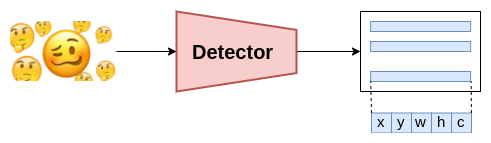
\includegraphics[scale=1.0]{images/model_architecture_target.png}}
	
	Некий детектор, который принимает на вход изображение, а выдает параметры каждого эмодзи.
	
	\textbf{Данные и оценка модели}\\
	Датасет может быть синтетическим и генерироваться на ходу. Несложно раскидать по изображению несколько эмодзи, и периодически добавлять шумы, искажения и лишние объекты. Также такая генерация даст разметку данных, что позволит оценивать модель (но разметка не будет использоваться для обучения).
	
	\textbf{Предлагаемая архитектура}\\
	Воспользуемся идеей автоэнкодера. В автоэнкодере есть энкодер, который переводит изображение в латентное векторное пространство, и декодер, который восстанавливает изображение из векторного пространства. Автоэнкодеры учатся выдавать то же изображение, что принимают на вход.
	
	\newpage
	То есть общий вид модели будет таким:
	
	\centerline{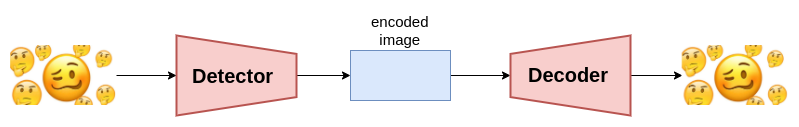
\includegraphics[scale=0.6]{images/model_architecture_general.png}}
	
	Но, так как мы решаем специфичную задачу: распознавание шаблонов, воспользуемся нетипичной схемой автоэнкодера. Возьмем в качестве энкодера модель распознавания объектов (Faster RCNN, SSD или YOLO). Таким образом, в нашем латентном векторном пространстве окажется список векторов, каждый из которых будет задавать:
	\begin{MyList}
		\item Координату центра баундинг бокса по оси X пропорционально изображению от $0$ до $1$. 
		\item Координату центра баундинг бокса по оси Y пропорционально изображению от $0$ до $1$.
		\item Размер баундинг бокса по оси X пропорционально изображению от $0$ до $1$.
		\item Размер баундинг бокса по оси Y пропорционально изображению от $0$ до $1$.
		\item Глубину объекта от $0$ до $1$ (для чего она нужна --- чуть позже).
		\item Распределение вероятности принадлежности объекта каждому из классов.
	\end{MyList}

	Декодер же будет делать очень простую вещь. Он для каждого класса объектов будет учить реальную картинку, то есть тензор, каждый элемент (пиксель) которого --- обучаемый параметр. Также декодер будет учить маску изображения, каждый пиксель которой задает прозрачность. Иными словами для каждого класса будет выучено RGBA изображение. Никаких других обучаемых параметров у декодера нет.
	
	Работа декодера --- чисто механическая:
	\begin{MyList}
	\item Для каждого найденного объекта выбрать класс, вероятность которого максимальна.
	\item По этому классу взять соответствующее ему изображение.
	\item Положить все изображения на белый фон, внутрь баундинг боксов, отмасштабировав и повернув.
	\end{MyList}

	Маска изображения нам нужна, так как распознаваемые объекты (эмодзи в данном случае) не прямоугольные, а имеют некую форму. Маска как раз задаст эту форму. А глубина объекта нужна, чтобы понять, в каком порядке класть маленькие изображения на общее. Это важно, так как они могут пересекаться.
	
	Декодер будет выглядеть так:

	\centerline{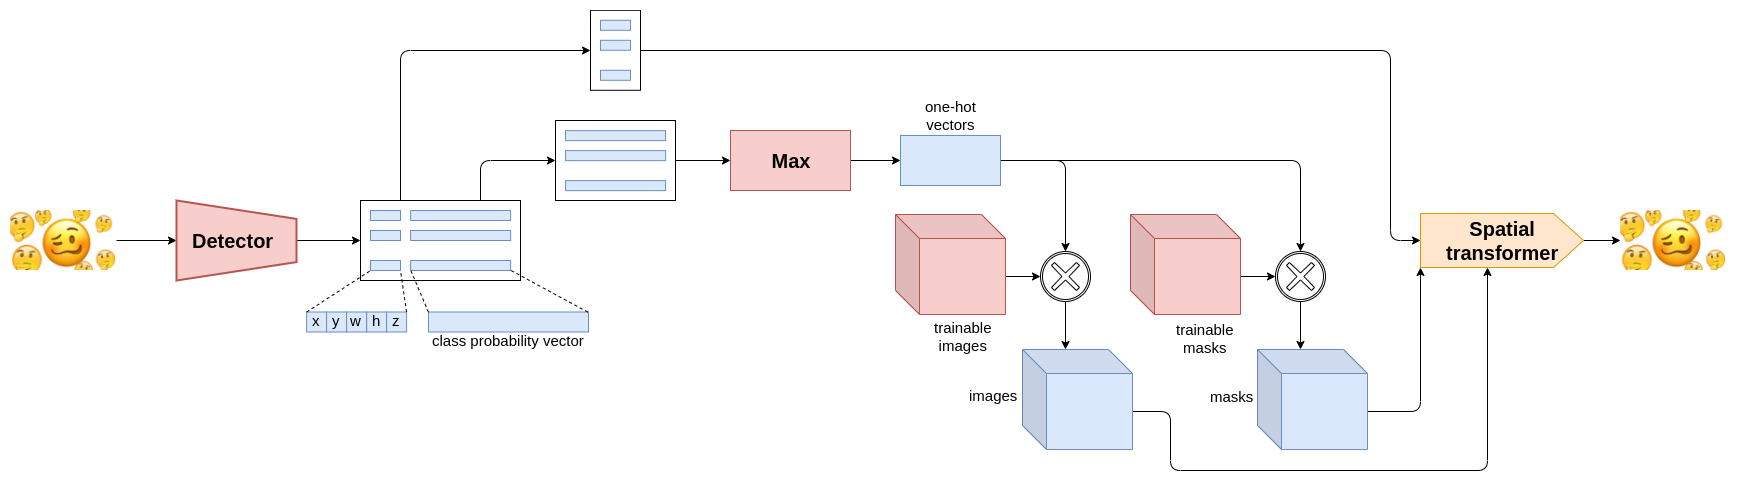
\includegraphics[scale=0.3]{images/model_architecture_decoder.png}}	
	
	\newpage
	\textbf{Обучение}\\
	Изначально модель можно обучать end-to-end, как обучается самый обычный автоэнкодер.
	
	Но вероятно здесь возникнут трудности с обучением детектора в режиме обучения end-to-end. Особенно в самом начале. Но предлагаемая архитектура удобна тем, что здесь можно провернуть следующий трюк.
	
	Пусть мы обучили модель end-to-end до какого-то состояния. Значит декодер выучил какие-то изображения, пусть даже очень плохие. Давайте возьмем эти изображения и сами сгенерируем размеченный датасет, точно также, как мы генерируем исходные данные для обучения, только воспользуемся картинками из декодера. А на размеченных данных легко обучить детектор, как это делается в обычном supervised object detection. 
	
	Такой трюк, особено вначале, поможет детектору определять одни и те же объекты на изображение, и тогда уже декодер сможет выучить шаблоны. Сделаем так несколько раз:
	\begin{MyList}
		\item Обучаем end-to-end.
		\item Обучаем только детектор по сгенерированным из декодера данным.
	\end{MyList}
	
	А под конец обучения можно сделать следующее:
	\begin{MyList}
		\item Зафиксируем детектор и распознаем много примеров.
		\item Получим много семплов каждого шаблона. Далее будем работать отдельно с каждым шаблоном.
		\item Посчитаем маску изображения руками так, чтобы непрозрачность каждого пикселя была пропорциональна дисперсии этого пикселя в семплах.
		\item Отфильтруем семплы объекта так, чтобы остались только те, которые похожи друг на друга (наименее зашумленные).
		\item Получим очень хорошие шаблоны. 
		\item Воспользуемся этими шаблонами для генерации данных и сделаем сильную аугментацию. 
		\item Обучим на этих данных детектор.
	\end{MyList}

	\textbf{Распределение работы}\\
	Этот поект предполагается на двух человек:
	\begin{MyList}
		\item Имплементирует детектор, организует процесс обучения.
		\item Имплементирует декодер, реализует генерацию данных по изображениям и аугментацию.
	\end{MyList}
	
\end{document}